\subsection{Mastering Ripple Measurement: The Best Oscilloscope Trigger Mode!}

\begin{tcolorbox}[colback=gray!10, colframe=black, title=E4A10] 

Which trigger mode is most effective when using an oscilloscope to measure a linear power supply’s output ripple?

\begin{enumerate}[label=\Alph*),noitemsep]
    \item A: Single-shot
    \item B: Edge
    \item C: Level
    \item D: \textbf{Line}
\end{enumerate} \end{tcolorbox}

\subsubsection{Concepts Related to the Question}

When measuring the output ripple of a linear power supply, it is crucial to understand the nature of the signal being measured and how the oscilloscope can effectively capture and display this signal. The ripple voltage is a small, periodic variation in the output voltage due to the rectification and smoothing processes within the power supply. 

An oscilloscope has various trigger modes, which can be used to stabilize and accurately display repetitive signals. The most relevant trigger modes are:

1. \textbf{Single-shot Trigger}: This mode captures a single event and can be useful for unique signals but is not optimal for continuous measurements like ripple.
   
2. \textbf{Edge Trigger}: This mode triggers on a transition in the voltage (rising or falling edge). While useful for many applications, it may not be ideal for steady-state ripple measurements.

3. \textbf{Level Trigger}: This mode triggers when the input signal crosses a predefined voltage level. It can be useful, but might be cumbersome for real-time monitoring of ripples which are continuous and small.

4. \textbf{Line Trigger}: This mode synchronizes the oscilloscope's sampling with the frequency of the AC line (typically 50/60 Hz). This allows the oscilloscope to lock onto the ripple occurring in the power supply, making it the most effective choice for measuring output ripple consistently over time.

\subsubsection{Conclusion}

Thus, the correct option for measuring ripple voltage of a linear power supply is option D: Line trigger. This method ensures you are triggering on a regular basis that correlates well with the operation of the power supply, allowing a clear view of the ripple in its natural context.

\subsubsection{Calculations and Diagrams}

If needed to analyze the ripple voltage quantitatively, you might measure peak-to-peak voltage of the ripple displayed on the oscilloscope. Suppose we observe a peak-to-peak voltage reading of 200 mV on the oscilloscope. 

The ripple voltage \( V_{ripple} \) can be calculated as:

\[
V_{ripple} = V_{max} - V_{min}
\]

where \( V_{max} \) and \( V_{min} \) are the maximum and minimum voltage levels of the observed ripple.

In this case:

1. Measure \( V_{max} = 1000 mV (1V) \)
2. Measure \( V_{min} = 800 mV (0.8V) \)

Thus, 

\[
V_{ripple} = 1000 \, mV - 800 \, mV = 200 \, mV
\]

In terms of visualization, below is a simple diagram using TikZ to illustrate a typical output ripple waveform observed across a linear power supply:

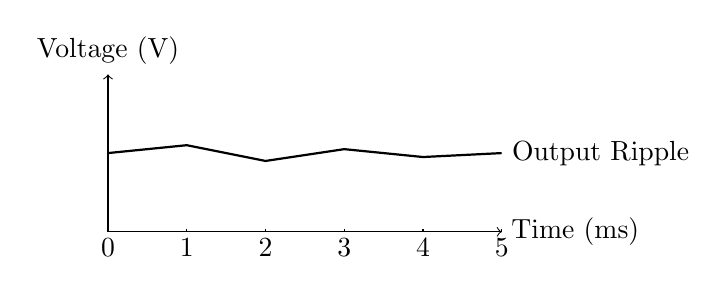
\begin{tikzpicture}
    \draw[->] (0,0) -- (0,2) node[above] {Voltage (V)};
    \draw[->] (0,0) -- (5,0) node[right] {Time (ms)};

    \draw[thick] (0,1) -- (1,1.1) -- (2,0.9) -- (3,1.05) -- (4,0.95) -- (5,1)
    node[right] {Output Ripple};

    \foreach \x in {0, 1, 2, 3, 4, 5}
        \draw[shift={(\x,0)}] (0pt,0pt) -- (0pt,1pt) node[below] {\x};
\end{tikzpicture}
